\section{Introduction}\label{sec:Introduction}

%%%%%%%%%%%%%%%%%%%%%%%%%%%%%%%%%%%%%%%%%%%%%%%%%%%%%%%%%%%%%%%%%%%%%%%%%%%%%%%%%
\subsection{Importance of drift velocity and electrict field determination}\label{sec:Intro}
%%%%%%%%%%%%%%%%%%%%%%%%%%%%%%%%%%%%%%%%%%%%%%%%%%%%%%%%%%%%%%%%%%%%%%%%%%%%%%%%%
The electron drift is the LArTPC working priciple. If we don't know the speed at which electron drift, we don't know their position on the direction of drifting, losing the 3D reconstruciton capabilities. The drift velocity determines the drift time. The more time electrons spend in the drift volume, the higher the probability they get caught in the argon electronegative impurities. This means that the drift velocity impacts the electron lifetime, which is fundamental to a proper calorimetric reconstruction. The drift velocity is determined by the electric field in the chamber. In what follows, we show (three) two methods to determine the electric field, drift velocity and drift time.

This note considers data from RunI and RunII only, since the quantites of interest for the analysis remained unchanged. The methodologies described can be applied to RunIII as well, $mutatis$ $mutandis$. 
\textcolor{red}{BLURB ABOUT WHAT IS IN WHAT SECTION}


%%%%%%%%%%%%%%%%%%%%%%%%%%%%%%%%%%%%%%%%%%%%%%%%%%%%%%%%%%%%%%%%%%%%%%%%%%%%%%%%%
\subsection{Definitions: electric field, drift velocity and drift time }\label{sec:Def}
%%%%%%%%%%%%%%%%%%%%%%%%%%%%%%%%%%%%%%%%%%%%%%%%%%%%%%%%%%%%%%%%%%%%%%%%%%%%%%%%%
LArIAT has 3 drift volumes: a main one between cathode and shield plane, and two smaller ones between shield and induciton planes (SI) and between induction and collection planes (IC). Scope of this work is to measure the electric field, drift velocity and drift time in the main drift volume using data.

For the data considered, we assume the voltages applied on shield, induction and collection planes are known and constants. Their value can be found in table \ref{tab:voltages}.
For RunI and RunII data, the spacing between both the shield and induction planes and the induction and collection planes is 4 mm. 

Table \ref{tab:Efields} reports the values of the electric field, drift velocity and drift times for the smaller drift volumes; the next few paragraphs describe how these quantities are calculated.  

The electric field is calculated using equation \ref{eq:Efield}:

\begin{equation} E_{field}=\frac{\Delta V_{ab}}{\Delta x}, \label{eq:Efield}
\end{equation}
where $\Delta V_{ab}$ is the voltage difference between two consecutive anode planes and $\Delta x$ is their spacing.

\begin{table}[b!]
\centering
\caption{Anode planes voltages}
\label{tab:voltages}
\begin{tabular}{lll}
\hline
\multicolumn{1}{|l|}{VShield} & \multicolumn{1}{l|}{VInduction} & \multicolumn{1}{l|}{VCollection} \\ \hline
\multicolumn{1}{|l|}{-298.75} & \multicolumn{1}{l|}{-18.5}      & \multicolumn{1}{l|}{338.5}       \\ \hline
                              &                                 &                                 
\end{tabular}
\end{table}



 
\begin{table}[]
\centering
\caption{Electric field and drift velocities in LArIAT smaller drift volumes}
\label{tab:Efields}
\begin{tabular}{|l|l|l|}
\hline
& Shield-Induction & Induction-Collection \\ \hline
E$_{filed}$ &                 700.625 V/cm        &                892.5  V/cm             \\ \hline
v$_{drift}$ &                   1.73  mm/$\mu$s   &                  1.90 mm/$\mu$s        \\ \hline
t$_{drift}$ &                   2.31  $\mu$s      &                   2.11 $\mu$s          \\ \hline

\end{tabular}
\end{table}

From the electric field, we calculate the drift velocity and substquently the drit time in the volumes bewteen shield and induction planes and induction and collection planes.
The relationship between drift time and drift velocity is straightforward 
\begin{equation}
v_{drift} = \Delta x/t_{drift}, \label{eq:drifttime}
\end{equation}
but the one between  electric field and drift velocity is more complicated. The relationship between the electric field and drift velocity in LAr can be described as 
\begin{equation} v_{d} = \mu(E_{field},T) E_{field}, \label{eq:vd}
\end{equation}
where where $\mu$ is the electron mobility in LAr and T the temperature. The electron mobility depends on the LAr temperature and the electric field. The empitical formula for this dependency is described in ~\cite{WWW} and shown in figure \ref{fig:EV} for several argon temperatures.


\begin{figure}[ht!]
\centering
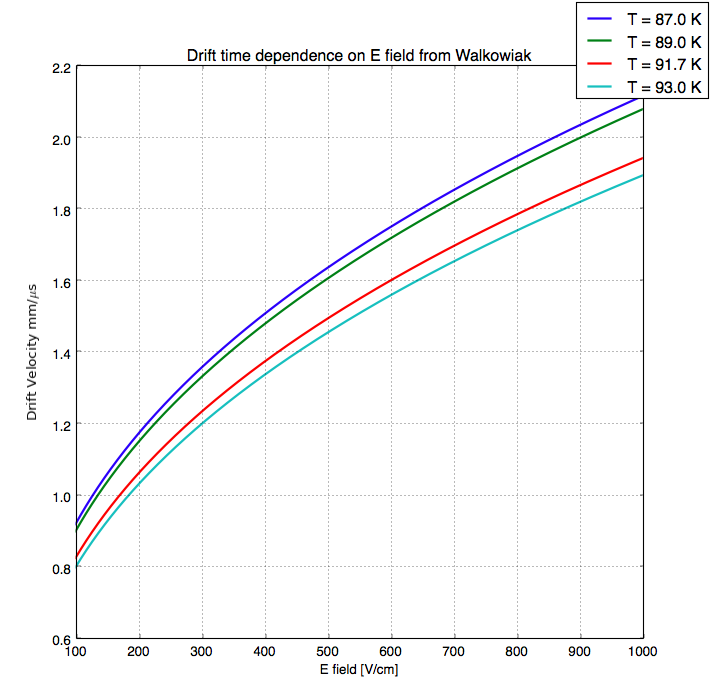
\includegraphics[scale=0.45]{./images/Walkowiak.png}\\
\caption{Drift velocity dependence on electric field for several temperatures.}
\label{fig:EV}
\end{figure}


In order to determine the temperature inside the TPC, we use the measurement of the pressure at the top of the cryostat. This pressure is maintained constant at ~20 psi at the liquid argon surface (PT219A in figure \ref{fig:cryo}). Figure \ref{fig:pressure} shows the distribution of the pressure reading for 13 days.
The average pressure is 20.0 $\pm$ 0.4 psi,  which corresponds to argon temperature of  90.328K  according to NIST RefProp [\textcolor{red}{reference}]. In order to calculate the pressure (and subsequently the temperature) in the middle of the TPC, we consider about 40 cm of Argon from the lulage surface. This argon raises the pressure of about 0.79 psi in the middle of the TPC. A pressure of ~20.79 psi corresponds to a temperature to ~90.7 K according to NIST. We'll assume a temperature of 90.7 K for the rest of the note.

It should be noted that LArIAT is equipped with three temperature probres inside the LAr: one at the bottom (TE213A in figure \ref{fig:cryo}), one in the middle (TE314A in figure \ref{fig:cryo}) and one on the top of the cryostat (TE212A in figure \ref{fig:cryo}). These probes have a similar temperature reading (see \ref{tab:temp}), but since they were not calibrated we prefer to rely on the pressure measurement.

 %\textcolor{red}{On average}, the three probes read as shown in table \ref{tab:temp}. 
\begin{table}[]
\centering
\caption{Average temperatures measured at the top, middle and bottom in the LArIAT cryostat.}
\label{tab:temp}
\begin{tabular}{|c|c|c|}
\hline
Top Probe Temp (TE212A) & Middle Probe Temp (TE214A)   & Bottom Probe Temp (TE213A)  \\ \hline
91.7 $\pm$ 0.7 K &  91.8 $\pm$ 0.7 K                   & 93.3 $\pm$ 2.7 K       \\ \hline
\end{tabular}
\end{table}


\begin{figure}[ht!]
\centering
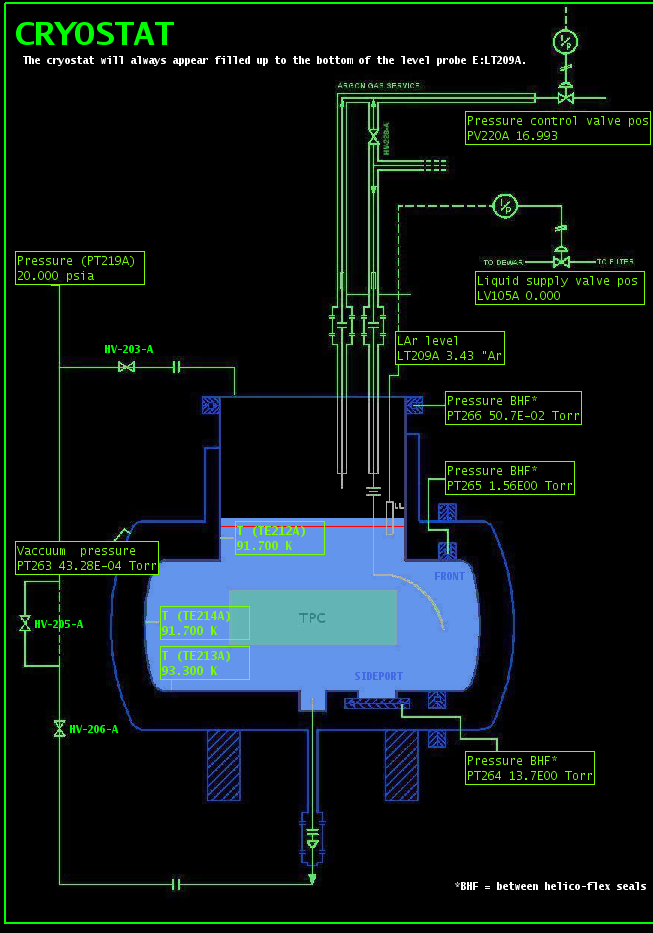
\includegraphics[scale=0.45]{./images/cryopic.png}\\
\caption{Scheme of LArIAT cryostat and cryo probes.}
\label{fig:cryo}
\end{figure}


\begin{figure}[ht!]
\centering
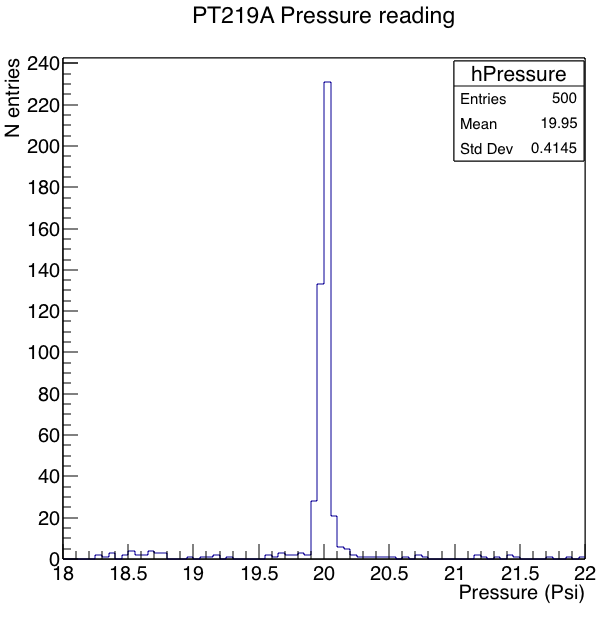
\includegraphics[scale=0.45]{./images/Pressure.png}\\
\caption{PT219A pressure distributions for 13 days (2017/6/23 - 2017/7/5).}
\label{fig:pressure}
\end{figure}





